\documentclass[preprint,10pt,nocopyrightspace]{sigplanconf}
% \documentclass{article}
\usepackage[T1]{fontenc} %%%key to get copy and paste for the code!
\usepackage[utf8]{inputenc} %%% to support copy and paste with accents for frnehc stuff
\usepackage{times}
\usepackage[scaled=0.85]{helvet}
\usepackage{graphicx}
\usepackage{ifthen}
\usepackage{xspace}
\usepackage{alltt}
\usepackage{latexsym}
\usepackage{url}            
\usepackage{amssymb}
\usepackage{amsfonts}
\usepackage{amsmath}
\usepackage{stmaryrd}
\usepackage{enumerate}

\usepackage[pdftex,colorlinks=true,pdfstartview=FitV,linkcolor=blue,citecolor=blue,urlcolor=blue]{hyperref}
\usepackage{xspace}
\usepackage{listings}


\newboolean{showcomments}
\setboolean{showcomments}{true}
\ifthenelse{\boolean{showcomments}}
  {\newcommand{\bnote}[2]{
	\fbox{\bfseries\sffamily\scriptsize#1}
    {\sf\small$\blacktriangleright$\textit{#2}$\blacktriangleleft$}
    % \marginpar{\fbox{\bfseries\sffamily#1}}
   }
   \newcommand{\cvsversion}{\emph{\scriptsize$-$Id: macros.tex,v 1.1.1.1 2007/02/28 13:43:36 bergel Exp $-$}}
  }
  {\newcommand{\bnote}[2]{}
   \newcommand{\cvsversion}{}
  } 


\newcommand{\here}{\bnote{***}{CONTINUE HERE}}
\newcommand{\nb}[1]{\bnote{NB}{#1}}

\newcommand{\fix}[1]{\bnote{FIX}{#1}}
%%%% add your own macros 

\newcommand{\sd}[1]{\bnote{Stef}{#1}}
\newcommand{\np}[1]{\bnote{Nico}{#1}}
\newcommand{\gd}[1]{\bnote{Gise}{#1}}

\graphicspath{{figures/}}
%%% 


\newcommand{\figref}[1]{Figure~\ref{fig:#1}}
\newcommand{\figlabel}[1]{\label{fig:#1}}
\newcommand{\tabref}[1]{Table~\ref{tab:#1}}
\newcommand{\layout}[1]{#1}
\newcommand{\commented}[1]{}
\newcommand{\secref}[1]{Section \ref{sec:#1}}
\newcommand{\seclabel}[1]{\label{sec:#1}}

%\newcommand{\ct}[1]{\textsf{#1}}
\newcommand{\stCode}[1]{\textsf{#1}}
\newcommand{\stMethod}[1]{\textsf{#1}}
\newcommand{\sep}{\texttt{>>}\xspace}
\newcommand{\stAssoc}{\texttt{->}\xspace}

\newcommand{\stBar}{$\mid$}
\newcommand{\stSelector}{$\gg$}
\newcommand{\ret}{\^{}}
\newcommand{\msup}{$>$}
%\newcommand{\ret}{$\uparrow$\xspace}

\newcommand{\myparagraph}[1]{\noindent\textbf{#1.}}
\newcommand{\eg}{\emph{e.g.,}\xspace}
\newcommand{\ie}{\emph{i.e.,}\xspace}
\newcommand{\etal}{\emph{et al.,}\xspace}
\newcommand{\ct}[1]{{\textsf{#1}}\xspace}
\newcommand{\cf}{\emph{cf.}\xspace}

\newenvironment{code}
    {\begin{alltt}\sffamily}
    {\end{alltt}\normalsize}

\newcommand{\defaultScale}{0.55}
\newcommand{\pic}[3]{
   \begin{figure}[h]
   \begin{center}
   \includegraphics[scale=\defaultScale]{#1}
   \caption{#2}
   \label{#3}
   \end{center}
   \end{figure}
}

\newcommand{\twocolumnpic}[3]{
   \begin{figure*}[!ht]
   \begin{center}
   \includegraphics[scale=\defaultScale]{#1}
   \caption{#2}
   \label{#3}
   \end{center}
   \end{figure*}}

\newcommand{\infe}{$<$}
\newcommand{\supe}{$\rightarrow$\xspace}
\newcommand{\di}{$\gg$\xspace}
\newcommand{\adhoc}{\textit{ad-hoc}\xspace}

\usepackage{url}            
\makeatletter
\def\url@leostyle{%
  \@ifundefined{selectfont}{\def\UrlFont{\sf}}{\def\UrlFont{\small\sffamily}}}
\makeatother
% Now actually use the newly defined style.
\urlstyle{leo}


\lstset{ %
  backgroundcolor=\color{white},   % choose the background color; you must add \usepackage{color} or \usepackage{xcolor}
  basicstyle=\footnotesize\ttfamily,        % the size of the fonts that are used for the code
  breakatwhitespace=false,         % sets if automatic breaks should only happen at whitespace
  breaklines=true,                 % sets automatic line breaking
  captionpos=b,                    % sets the caption-position to bottom
  escapeinside={\%*}{*)},          % if you want to add LaTeX within your code
  extendedchars=true,              % lets you use non-ASCII characters; for 8-bits encodings only, does not work with UTF-8
  keepspaces=true,                 % keeps spaces in text, useful for keeping indentation of code (possibly needs columns=flexible)
  numbersep=5pt,                   % how far the line-numbers are from the code
  rulecolor=\color{black},         % if not set, the frame-color may be changed on line-breaks within not-black text (e.g. comments (green here))
  showspaces=false,                % show spaces everywhere adding particular underscores; it overrides 'showstringspaces'
  showstringspaces=false,          % underline spaces within strings only
  showtabs=false,                  % show tabs within strings adding particular underscores
  stepnumber=2,                    % the step between two line-numbers. If it's 1, each line will be numbered
  tabsize=2,                       % sets default tabsize to 2 spaces
}

\lstdefinelanguage{Wollok}{
  keywords={program, console},
  sensitive=true,
  comment=[l]{//},
  morecomment=[s]{/*}{*/},
  morestring=[b]',
  morestring=[b]"
}


\begin{document}
\title{Wollok -- Relearning How To Teach Object-Oriented Programming}
\authorinfo{Nicolás Passerini}
  {UTN -- Facultad Regional Buenos Aires \\ Universidad Nacional de Quilmes \\ Universidad Nacional de San Martín}
  {npasserini@gmail.com}
  
\authorinfo{Javier Fernandes}
  {Universidad Nacional de Quilmes \\ Universidad Nacional de San Martín}
  {javier.fernandes@gmail.com}
  
\authorinfo{Pablo Tesone}
  {Universidad Nacional de Quilmes \\ Universidad Nacional del Oeste \\ Universidad Nacional de San Martín}
  {tesonep@gmail.com}

\date{\today}
\maketitle

\begin{abstract}
In this context...
We consider this problem P...
P is a problem because...
We propose this solution...
Our solution solves P in such and such way.
\end{abstract}

\section{Introduction}
\label{sec:intro}

% Context
% (a) hay que arrancar introduciendo nuestra visión, contando por qué enseñamos objetos de determinada manera, por qué hicimos Ozono.

% La importancia de arrancar con objetos. -- No sé si arrancar con esto.
\emph{Object-oriented programming} (OOP) has become the \textit{de facto} standard programming paradigm in industrial software development.
Therefore, in the last years software engineering curricula have put more emphasis in object-oriented courses.
% Furthermore, opinion in the community is divided as if it should be the first programming model to be presented. 
% Problem
Still, students often have difficulties in learning how to program in an object-oriented style which show up both in academic and in industrial environments.

Several causes have been blamed for the difficulties in OOP learning.
First, OO courses tend to focus too much on syntax and the particular characteristics of a language, instead of focusing on OOP distinctive characteristics.
Second, many OO languages used in introductory courses do require to grasp a lot of quite abstract concepts before being able to build a first program.
Finally, poor programming environments are used, although we are at a time where an unexperienced programmer could be making great use of the guidance a good programming environment could provide.
\np{En realidad algunos de estos problemas no son exclusivos de OOP, habría que ver si queremos decir algo al respecto.}

\medskip 

% Known tracks for solutions
% here you want to show that you are not an idiot not knowing what have been around

% Primero hablar de lenguajes específicos para enseñar
There have been several proposals to address the difficulties in introductory OO courses 
by defining a specific language which provides a simplified programming model such as Karel++ \cite{bergin_karel++:_1996} \np{¿otros?}.
This approach has been used even outside the OO world \cite{feurzeig_programming-languages_1970, pattis_karel_1981, lopez_nombre_2012}.
% Environments
A step further is to provide a whole programming environment specifically designed to aid novice programmers 
such as Squeak \cite{ingalls_back_1997}, Traffic \cite{broy_outside-method_2003} and BlueJ \cite{bennedsen_bluej_2010}. 

% Object first
The great differences between these programming languages and environments show that they have to be analyzed in the light of the pedagogical approaches behind them.
The tools are of little use without this pedagogical view.
For example, some educational languages and environments are designed to be used in \textit{object-first} approaches, 
\ie for students without any previous programming knowledge \cite{arnow_introduction_1998, bruce_library_2001}.
% Children
Other languages are focused on teaching to children or teenagers, such as Scratch \cite{malan_scratch_2007} and Etoys \cite{lee_empowering_2011}. 
% Visualization
Finally, there are many approaches which emphasize the importance of \emph{visualization tools} 
to simplify the understanding of the underlying programming model \cite{cooper_teaching_2003, roberts_designing_1998}.

\medskip
% Nuestro trabajo

Previous works from our team \cite{lombardi_instances_2007,lombardi_carlos_alumnos_2008,griggio_programming_2011,spigariol_lucas_ensenando_2013} have described an approach consisting of
(a) a novel path to introduce OO concepts, focusing on objects, messages and polymorphism first, while delaying the introduction of classes and inheritance and 
(b) a reduced and graphical programming environment which supports the order in which we introduce the concepts, by allowing to build OO programs without the need of classes.
Our approach focuses on the concepts of object, message, reference and object polymorphism, while delaying the introduction of more abstract concepts such as types, classes and inheritance.
These way of organizing a course provides a more gentle learning curve to students and allows them to write completely working programs from the first week.

% What our solution is \ct{Set} and \ct{OrderedCollection} (so that the reader knows where the paper is going)
% Contribution of the paper
% (b) lo que aprendimos en estos 8 años haciendo eso, que nos lleva a querer darle una vuelta más.
While this approach proved to be successful in providing the students with a more profound knowledge of OOP at the same time as raising pass rates, 
we feel that there is still room for improvement, in four areas:
(a) integrating object-based and class-based programs together,
(b) creating automatic ways to produce a graphical user interface (GUI),
(c) enhancing the programming environment with a type inference tool that helps avoiding some common mistakes
and (d) narrowing the distance between our language and tools with those more frequently used in industrial development.

\np{No sé si hablar de los temas de colecciones, son un poco particulares de Ozono.
También del environment se podrían decir más cosas que sólo el sistema de tipos.}

\medskip 
% Paper structure
\np{falta paper structure}


\section{Problem Description}
\label{sec:problem}

% Context, exposed with the \textbf{most precise terms possible} (don't open
% unwanted doors for the reader)

% Los cursos se enfocan en sintaxis y usan lenguajes inadecuados.
On cause behind the difficulties in learning OOP is that courses often focus on syntax and the particular characteristics of a
programming language, leading students to concentrate on these relatively unimportant details rather than the underlying object-oriented modelling skills. 
Also, the use of industrial languages to introduce OOP requires the student to understand several concepts before being able to run his first program.

% Ejemplo con Java.
By focusing on those details, many students fail to comprehend the essential model that transcends particular programming languages \cite{the_joint_task_force_on_computing_curricula_computing_2001}. 
Figure \ref{fig:helloWorld} shows a typical first program, written in Java \cite{arnold_java_1996}.
To get this program running, the student has to walk through a minefield of packages, classes, scoping, types, arrays and class methods among other complex concepts.
However, he is still not able to do more basic OO programming, such as sending a message to an object.

\begin{figure}[h]
 \centering
 \begin{lstlisting}[language=Java]
	package examples;
	
	public class HelloWorld {
		public static void main(String[] args) {
			System.out.println("Hello World");
		}
	}
 \end{lstlisting}
 
 \caption{\small Sample initial Java program which diverts student attention from the most important concepts.}
 \label{fig:helloWorld}
\end{figure}

% Por eso los pibes no aprenden
For all these reasons, courses tend to spend too much time concentrated on the mechanistic details of programming constructs, 
leaving too little time to become fluent on the distinctive characters of OOP, 
such as identifying objects and their knowledge \emph{relationships}, assigning \emph{responsibilities} 
and taking advantage of \emph{encapsulation} and \emph{polymorphism} to make programs more robust and extensible.

% Además necesitamos environments
To make things worse, frequently the students do not have proper tools that could help them overcoming all the obstacles.
Already in 1999, Kolling \etal had established the importance of enviroments in introductory courses \cite{kolling_problem_1999}. 
He stated that earlier introductory courses focused on the development of algorithms in procedural or functional languages. 
To do this, an editor and a compiler was all that was needed for the practical part of the work. 
Modern courses now use object-oriented languages and subject material taught includes testing, debugging and code reuse. 
This creates the need to deal with multiple source files and multiple program development tools from the very start. 
To give a beginning student a chance to cope with this increased complexity, better environment support is needed. 

\medskip

% Probably set the vocabulary before to cut any misinterpretation
% Problem

% Consecuencias en la acadamia y en la industria
The failure of students to understand the essential object-oriented concepts shows both in academy as in industry.
In academic environments we find very low completion rates in introductory OO courses.
Moreover, students in their very beginning of an informatic carreer which fail their introductory programming courses, are often likely to give up their studies\np{cite needed}.
In industrial development, we find that these hindrances reduce the opportunity of students to apply
the concepts of the paradigm effectively in their further
professional practice, resulting in several IT-projects not taking
advantage of the possibilities offered by the potential of good
object-oriented practices. \cite{lombardi_instances_2007}

\medskip 

% Factual solution tracks, to position...
\np{Contar algo de otras propuestas anteriores a la nuestra}

Our previous work in this area is based on the proposal to change the order of subjects in OOP introductory coures \cite{lombardi_instances_2007}.
To enable this we provide a simplified OO language with an ad-hoc educational programming environment 
named Ozono\footnote{The name has been changing along these years. Other names for our programming enviroment have been ObjectBrowser, Loop and Hoope}, 
in which students can create objects and define their behavior directly, without the need for classes and inheritance \cite{griggio_programming_2011}.
Ozono is based on Smalltalk\footnote{The latest version currently in use in universities is based on a Smalltalk dialect named Pharo \cite{black_pharo_2010}.}.
and thus it is a \textit{dynamic language}.

We take special advantage of the dynamic characteristic of the language because it allows very simple uses of polymorphism, 
\ie any two objects that understand a common set of messages can be treated polymorphically without worrying about inheritance or \emph{interface} implementation.
This enables the students to exploit polymorphism already in their programs after only two or three weeks of the course.
\np{Qué otras ventajas queremos contar?}

\medskip
This approach produced impressive results and therefore has been adopted in other courses and universities.
The simplified programming model, allows the students to spend more time working with the essential concepts of the OO paradigm.
This, in turn allows for more practice and more complex exercises, even incorporating more advanced OO techniques such as \emph{design patterns} \cite{Gamm03a},
which in traditional approaches are normally postponed to a second OOP course.

% Esto podría extender la descripción del problema
%  Ozono hereda muchos de los problemas de los entornos Smalltalk

% Smalltalk, however, lacks other important facilities: no visualisation tools for class
% relations are available. The main problem with this lies in the Smalltalk language 
% itself: since it is not statically typed, it is not possible to extract usage relations fromo
% its source code. No indication exists before runtime as to the call relationships
% between classes. Inheritance relationships as shown in the browser do not present
% the relationships of one application but rather the whole Smalltalk environment and
% so the browser is not used as an application modelling tool. .
% Reports about the use of Smalltalk systems for teaching also point to another
% problem: its size. While the language itself (in terms of the number of constructs) is
% small, the class library and tools are large and often confusing. Several authors
% reported difficulties with the students ability to cope with the environment [7, 8],
% especially that experimentation and self directed learning was not working well
% because students were overwhelmed by the system. They also found that the
% functionality of the browser should be limited, since its power and flexibility caused
% more problems than it solved. \cite{kolling_problem_1999}.


% Our solution in a nutshell.
% (c) las ideas nuevas... y wollok como herramienta para dar soporte a esas ideas.

% Our solution: approach
Still, the experience of eight years in four universities\footnote{Ozono is currently used in Universidad Tecnológica Nacional, F.R. Buenos Aires and F.R. Delta, 
Universidad Nacional de Quilmes, Universidad Nacional de San Martín and Universidad Nacional del Oeste.}
and thousands of students has provided us with new insights of the learning process, 
which is what lead us to introduce several adjustements in our approach.

In the first place, starting with a \emph{classless} language mandates a change of language and enviroment in the middle of the course,
which is confusing for some students. 
To solve this, we propose to integrate \emph{class-based} and \emph{self-defined} objects in the same language.
\np{Ver bien qué nombres les ponemos y definir los conceptos antes.}
\np{En algún lugar decir que algunos lenguajes modernos hacen eso, como Scala.}

Second, we think that the absence of static typing information (which Ozono inherits from Smalltalk) prevents our programming environment to aid the students in finding some typical beginner mistakes.
Still, we do not want to force the students to add type annotations to their code, because that would distract them from the concepts we want to focus on.
We propose to settle this apparent controversy by enhancing our programming environment with a type inferer.
By doing so, the student is not required to care about type annotations, and at the same type we can detect some programming mistakes and aid the student in solving them.

Last, we have detected that sometimes the students which seem to understand the main concepts and can apply them in interesting ways to create medium to complex program, 
then have a hard time translating this knowledge to their professional activity.
We think that a good mitigation plan for this problem starts with bringing the activities in the course as close as possible to the professional practice.
For that matter, we propose to incorporate industrial best practices such as code repositories and unit tests, adapted to the possibilities of students with little or no programming experience.

\medskip
% Our solution: environment
The renewed approach is supported with a new programming language, named Wollok, and a programming environment which aids students to write, test and run programs.
Wollok is designed to give support to our pedagogical approach; 
it allows to define both classes and standalone objects,
incorporates a basic type inferer
and provides a simple syntax to define unit tests.

A big difference with Ozono and other educational OO languages is that Wollok is a \emph{file-based} language.
While we recognize the value of the \emph{image-based} approaches, we also are aware that most industrial programming enviroments are file-based.
Therefore, we think that a file-based approach will shorten the distance between the classroom and the professional activity, which is one of our main goals.
Moreover, image-based enviromnents tend to blur the distinction between the programming environment and the program under development,
which can embody great possibilities for advanced programmers but often does not more than confuse beginners.
Also, being file-based, Wollok allows for integration for the most popular code repositories.

Finally, the programming enviroment incorporates several advanced characteristics from professional environments, 
which improves the coding experience, and at the same time allows the student to familiarize himself with the kind of tools he will face in his later professional activity.
For that matter, the enviromnent incorporates content assist, automatic refactorings, advanced code navigation, 
language semantics-aware search tools and error highlighting \emph{while-you-type}

\medskip
% Contribution
It is important to notice that neither the Wollok language nor the programming environment contain novel features that are unseen in intustrial tools.
Therefore, the distinctive characteristic of these tools is the search for a programming environment which 
(a) supports our pedagogical approach,
(b) feeds the student with a set of tools which are adequate to his current knowledge
and (c) gently prepares him to be using industrial-level tools.

A big amount of effort in our research has been put in looking for solutions that can solve the apparent controversy between the last two objectives.
Often, the rich set of tools an industrial language or programming environment offers, cannot be exploited by an unexperienced programmer or even confuses him.
On the other end, we think that poor programming enviroments fail to help the students to make his first steps in programming and so trims the possibilities of introductory courses.
Therefore, there is much to gain from a language that has the exact features a teacher wants to teacher
and a programming enviroment which provides the exact tools a student can take advantage off at each time of his learning process.

% Constraints that influenced the solution (because the solution is not
% universal) \emph{e.g.} our requirements for a solution, possibly not all
% satisfied. They should be sound and believable. Analysis of the criteria.
% Imagine that you are another guy having this problem do the constraint
% matches yours so that you could apply the solution
\np{Esto tenía ganas de decir pero no me doy cuenta dónde ponerlo... no sé si volarlo y ya.}
So far we have focused on university students which have had a previous subject on inperative programming.
It is a pending job to adapt these ideas to teenagers or more generally students without any prior programming experience.

\section{Wollok: The Language}
\label{sec:wollokLanguage}

% Free form, variable number of sections, technical details.
% But in general do not mix solution and discussions/possible variation let that for discussion

Wollok is a brand new language, built to specifically give support to our pedagogical approach.
Many ideas have been inherited from our previous projects, such as Ozono or Loop. 
The most important of these inherited characteristics is the ability to create objects and treat them polymorphically without the need of type annotations, classes or inheritance.
Also, as its predecessors and unlike other pedagogical tools, Wollok is a \emph{general purpose} language, \ie it is not tied to any specific domain.

\medskip
One of the main objectives of building a new language is to provide a smoother transition from the first phase of the course,
in which students use a simplified programming model and the second phase, in which they use a full-fledged OOP language.
With our previous programming tools students were required to discard, in the middle of the course, the programming model and enviromnent they already knew and were used to.
This transition has sometimes been traumatic, because the process to define an object has to be re-learnt and the tools they had been using up to that point are no longer available.
With our new approach, the tools they first learnt are going to continue being available through all the course, together with the new ones that are incorporated in later lectures.
This is also consistent with some modern industrial OO languages that allow to define both classes or standalone objects, such as Scala \cite{Oder04a}.

\medskip
Also we reduced to a minimum the syntax and the most basic constructs of the language.
While this objective was already present in our previous work, the implementation strategy of Wollok allows us to go much further in accomplishing this goal, \cf Sec. \ref{sec:implementation}.
The example in figure \ref{fig:helloWorld/wollok} shows how the classical hello world would look in Wollok.
To build this first program students are not required to know about typing, scoping or packaging.
The only required construct is the \lstinline[language=Wollok]{program} and the only command is a message send.
Both the receiver and the parameters are built-in objects which will be handled in the same way as user-defined objects.
The concepts required to understand this program are no more than program, object, message and argument passing.

\begin{figure}[ht]
 \centering
 \begin{lstlisting}[language=Wollok]
	program {
		console.println("Hello World!")
	}
 \end{lstlisting}
 
 \caption{\small Sample initial Wollok program.}
 \label{fig:helloWorld/wollok}
\end{figure}

\medskip
% Effect
\np{Esto requeriría una mención en la intro, o en general una explicación más detallada.}
Another concept we propose to emphasize in the first programming courses is the control of side effects, 
\ie a programmer should be aware of the potential side effects of each portion of code.
The most basic feature in Wollok to control side effects is the ability to 
differentiate variables (defined using \lstinline[language=Wollok]{var})
from constants (defined using \lstinline[language=Wollok]{val}).
One step forward is to incorporate an \emph{effect system} \cite{nielson_type_1999}, \cf Sec. \ref{sec:furtherWork}.

\medskip
% Misceláneos
% Profundizar y pulir el highlighting the conceptos primarios y la estratificacion de conceptos
To sum up, there are several simple features which help structure the way a student sees his programming activity.
\emph{Object literals} and \emph{collection literals} reduce boilerplate on object creation, 
since we think that the excess of bureaucracy to create an object helps to build up 
the belief that using objects or collections is far more complicated than using numbers or strings, which in turns leads to \emph{primitive obsession} \cite{fowler_refactoring:_1999}.
% Objetos no como un elemento de la IDE -Ozono: nueva referencia global, sino como un elemnto del lenguaje. Evita referencias globales.

Each Wollok file has to be defined as \emph{program}, \emph{library} or \emph{test}.
Only programs and tests can be run. Libraries can only be \emph{imported} from programs, tests or other libraries.
This concepts push students onto modularizing their programs into smaller units that can be reutilized.

Figure \ref{fig:polymorphism} shows some of the mentioned features.
The programs includes two objects which are treated polymorphically, collections and block closures.
Students should be able to build such a program after four lectures.
In the first lecture we introduce objects, messages, methods and references;
in the second one we focus on polymorphism;
and in the following two we work with blocks and collections.

\np{Acá falta hablar de la diferencia entre objeto y referencia}

\begin{figure}[ht]
 \centering
 \begin{lstlisting}[language=Wollok]
	program myProgram {
		val optimistic = object {
			method hiThere() {
				"Hi, what an amazing day !"
			}
		}

		val pessimistic = object {
			method hiThere() {
				"Don't talk to me, it's a terrible day!"
			}
		}
		
		val all = #[optimistic, pessimistic]
		
		console.println(all.map[p| p.hiThere()])
	}
 \end{lstlisting}
 
 \caption{\small Simple polymorphism example.}
 \label{fig:polymorphism}
\end{figure}


\section{A Customized Programming Environment}
\label{sec:environment}

Beginner programmers are likely to require more guidance and make more mistakes than experienced programmers.
Therefore, we think that is much to gain from a good programming environment which structures the programming experienced and helps the students to identify common mistakes.

% \subsubsection{Visualización y Navegación}
% \begin{itemize}
%   \item syntax highlight
%   \item outline
%   \item hovering
%   \item vista de problems 
%   \item navigate: goto (F3, click), flechita para ir al método que sobrescribe.
%   \item find references 
% \end{itemize}
% 
% \subsubsection{Asistencia}
% \begin{itemize}
%   \item content assist
%   \item quick fixes
%   \item code templates (nuevo)
% \end{itemize}
The Wollok programming environment includes a lot of features that provide guidance to the student.
\emph{Content assist} shows the students what are his possibilities at any moment and feeds automatically into the code the most usual constructs, 
allowing the student to concentrate less on syntax and more in the modelling of the exercise problem.
\emph{Quick-fixes} allow Wollok not only to highlight problems in the student's code but also to propose automatic solutions for some usual mistakes.
\emph{Advanced code navigation} and \emph{smart reference searches} allow the programmer to better understand the dependencies in his program.
\np{¿Se les ocurre cómo mejorar eso?}
Moreover, \emph{automatic class diagrams} provide a high level view of the program and also helps understanding.

% Detect mistakes
Also, the programming environment has many tools intended to help detecting mistakes, even while the student is writing code.
\emph{Syntax highlighting} helps identify the most simple mistakes by providing immediate feedback when something is not right. 
Moreover, the enviromnent provides \emph{real-time highlights} for syntactic mistakes.
Finally, the \emph{type inferer} allows to detect more subtle mistakes.
All these tools allows the student to gain more control of his code, keeping him away from feeling lost, 
which is otherwise a common situation for a student walking his first steps into programming.

% Este no sé cómo ponerlo, es muy crítica al smalltalk.
% 8-reducir errores frustrantes: se cancela la edicion por tener 1 solo editor de metodo por ves (poder visualizar más que un sólo método simul), evitar errores de imagenes)

\medskip
% Type inferer
The type inferer is one of the most distintive characteristics of the Wollok programming environment.
We think that type inference is key to a simple programming environment.
On one side, it allows to detect lots of common mistakes \emph{before running the program}:
if an object does understand a message, if a wrong argument is passed, if incompatible types are mixed or even miss-spellings.
In enviroments without this capability it takes more time to detect errors.
Moreover, it is not uncommon that a type mistake produces a runtime error in a place different from where the mistake was done, producing confussion.

Still, providing a type inferer for a language such as Wollok has many subleties, which deserves an independent study \cite{type inferer}.
On one side we require it to be able to work without type annotations and at the same time provide feedback useful for an unexperienced programmer.
On the other side, the type system is rather complex;
for example, the presence of stand-alone objects requires the type system to handle \emph{structural types}, since a named type system would not allow them to be treated polymorphically.
Also, we want to be able to treat polymorphically stand alone objects with class-based objects.

\subsubsection{Checkeos y validaciones}
 
Todos los checkeos y problemas
generados se muestran agrupados en una vista dedicada a tal fín (Problems).

% En lo que sigue fui comentando las cosas que ya están dichas pero no quiero borrar esta enumeración porque está muy buena.
\begin{itemize}
%   \item \textbf{De sintaxis}: dados por el parser y lexer automáticamente.
  \item \textbf{De estilo}: para promover uniformidad y consistencia de código.
  Ejemplos:
  		\begin{itemize}
  			\item \textit{Nombres}: variables camelcase comenzando en minúscula,
  			nombres de clases camelcase iniciando mayúscula, packages en minúsculas, etc.
  			\item \textit{Orden y agrupamiento}: dentro de un objeto o clase, primero
  			se definen sus referencias internas, luego constructores y finalmente los métodos.
  			\item \textit{Separación de programas}: las clases sólo se pueden definir
  			en archivos de tipo \textit{librería}, no dentro de un \textit{program}.
  			\item \textit{Evitar referencias duplicadas}: no se puede definir una
  			referencia con nombre ya utilizado en alguna otra referencia del contexto (local, método,
  			clase/objeto, etc.). Ni tampoco si ya está definida en la superclase.
		\end{itemize}
  \item \textbf{De resolución de referencias}: para evitar referencias a
  variables inexistentes y, en la medida de lo posible (por ser de tipado
  implícito) de envío de mensajes. Ejemplos:
  		\begin{itemize}
		  \item \textit{Referencias inexistentes}: a variables locales, parámetros, o
		  internas (clase/objeto).
		  \item \textit{Constructores inexistentes}: evaluando existencia de la
		  clase, y compatibilidad en el número de paråmetros.
		  \item \textit{Envío de mensajes (a this)}: al ser a this se pueden realizar
		  checkeos por la existencia del método y compatibilidad de parámetros, incluso sin
		  involucrar al sistema de tipos.
		\end{itemize}
  \item \textbf{De uso de referencias}: para la detección de código
  	erroneo o bien desactualizado. Por ejemplo: warnings por referencias nunca
 	utilizadas, nunca asignadas, o utilización de variables en lugar de valores.
  \item \textbf{De estructura}: evitan por ejemplo inconsistencias en las
  estructuras creadas por el alumno. Por ejemplo, se checkea
  que un método marcado como \textit{override} efectivamente esté
	sobrescribiendo.
  \item \textbf{De tipos}: verifican compatibilidad de referencias en base a sus
  tipos. Por ejemplo ante envío de mensajes, o asignaciones de variables. Basado
  en el sistema de tipos.
\end{itemize}

\np{override}


\section{Discussion}
\label{sec:discussion}

% Discussion of actual solution \emph{vs.} initial constraints from \ref{sec:problem}. Explain the space of the solution, why we made it this way.
There are number of discussions that arised while evaluating the experiences
with our previous tools in courses, and that were taked into account in Wollok's
design.

One of them is whether the learning experience should provide a way to reuse
code while still in the form of pure objects without classes.
We detected that while working only with objects, on the first part of the
course, it's common to end-up with excersices where there will be at least some
sort of duplicated code between objects.
On this matter Ozono provided a mechanism based on prototypes, similar to that
found in Self language\cite{Ungar87self:the, Ungar91organizingprograms}. That
allowed full reuse of code (both behavior and state).
On the other hand, contrarily to what we suspected while designing Ozono, we've
found that in practice, introducing prototyping didn't smooth the transition
between objects and classes. Actually it made it harder.
In addition, prototyping is an excellent abstract model for pure object
languages, keeping it simple and incredible powerful. But there are almost no popular or industrial
languages implementing it (besides Javascript which is not exactly as standard
Self prototyping). 


So Wollok doesn't provide any form of inter-object reusage (besides classes).
When duplicated code appears as part of the course, it's important to
highlight that to students, and delay solving code duplication later with
classes.

\medskip


Se podría hablar de la discusión sobre si proveer formas de compartir comportamiento sin clases, como clonado.
También de la necesidad de crear colecciones independientemente, aunque es un poco específico de Ozono.

\medskip
Acercar la experiencia de aprendizaje a las prácticas industriales: 
(acá el palo de que la imagen sólo existe en smalltalk, y en la industria nadie la usa. 
Atrás de eso, la idea de archivos, y poder compartir con SVC. Por último la idea de actualizarse a un lenguaje con influencia de lenguajes modernos como xtend, scala, ruby, etc.)


% Evaluation of the solution. How does the solution meet the criteria? Where does it succeed or fails...


\section{Related Works}
\label{sec:related}

% Other solutions in the domain, and a real comparison of our contribution with solutions from other people.

% Agregar referencia al paper de Fidel, y otros

% Base tomada del paper de ESUG 2011
LOOP is presented as a visual environment to teach OOP using
a reduced set of language constructions and a prototype approach
to create objects. It presents the main concepts of object, message
and reference in a specialized tool with a visual representation of
the object environment. Several visual tools to teach programming
already exists, like ObjectKarel[2], Scratch[14] and Etoys[4].
ObjectKarel presents a visual tool based on the abstraction of
robots to teach OOP, using a map where the robots-the objects-
move when messages are sent to them. LOOP does not center on a
specific abstraction like a robot: it allows the student to create any
other abstraction. Scratch and Etoys, are aimed to teach the basics
of programming to children, using visual objects and scripts to play
tween objects. This kind of diagrams could be inferred from the
evaluation of any piece of code, even the execution of tests.
Another subject of research is a “debugger” for the tool [1]. We
think that a live and powerful debugger a ` la Smalltalk is a rich tool
for the understanding of the whole environment behaviour. After a
message is sent, a debugger view can be used like a video player,
with play, forward and backward buttons to navigate the message
stack and see how the state changes after each message send in the
object diagram.
Finally, there are some improvements to be made to the user
interface, such as shortcuts, code completion, improved menus or
internationalization. Currently the tool is only available in spanish,
we want to make it configurable to add more languages as neces-
sary.

In response to interest in an objects-first approach, several
texts and software tools have been published/developed that
promote this strategy (such as [1, 12]). Four recent software
tools are worthy of mention as using an objects-first
approach: BlueJ [9], Java Power Tools [11], Karel J. Robot
[2], and various graphics libraries. Interestingly, all these
tools have a strong visual/graphical component; to help the
novice “see” what an object actually is – to develop good
intuitions about objects/object-oriented programming.
BlueJ [9] provides an integrated environment in
which the user generally starts with a previously defined set
of classes. The project structure is presented graphically, in
UML-like fashion. The user can create objects and invoke
methods on those objects to illustrate their behavior. Java
Power Tools (JPT) [11] provides a comprehensive,
interactive GUI, consisting of several classes with which 
the student will work. Students interact with the GUI, and
learn about the behaviors of the GUI classes through this
interaction. Karel J. Robot [2] uses a microworld with a
robot to help students learn about objects. As in Karel [10],
Robots are added to a 2-D grid. Methods may be invoked
on the robots to move and turn them, and to have the robots
handle beepers. Bruce et al. [3] and Roberts [13] use
graphics libraries in an object-first approach. Here, there is
some sort of canvas onto which objects (e.g. 2-D shapes)
are drawn. These objects may have methods invoked on
them and they react accordingly.
In the remainder of this paper, we present a new
tactic and software support for an objects-first strategy. The
software support for this new approach is a 3D animation
tool. 3D animation assists in providing stronger object
visualization and a flexible, meaningful context for helping
students to “see” object-oriented concepts. (A more detailed
comparison of the above tools with our approach is
provided in a later section.) \cite{cooper_teaching_2003}

\section{Conclusion}
\label{sec:conclusion}

% In this paper, we looked at problem P with this context and these
% constraints. We proposed solution S. It has such good points and such not so
% good ones. 


Wollok is an educative, object-oriented programming language which is accompanied by an advanced programming environment.
Both tools are highly customized to give support to an introductory OOP course.
Our approach consists of the combination of these three cornerstones.

First, an \emph{incremental\np{Revisar la idea de Javi} learning path} choosing exactly which are the concepts we want to teach and the order we want to teach them.
The learning path starts with a \emph{simplified programming model} (SPM), \ie one which uses less concepts than a full-fledged OOP language.
The SPM allows the student to build simple programs without requiring more advanced concepts.
The path should attach the SPM with a good set of programming exercises, specifically oriented to be easy to build in the selected SPM.
Once the student has mastered the concepts on the SPM, we can go a step further and introduce the next set of concepts.
\np{Acá se podría hablar de constructivismo.}

Next, defining our own programming language, allows us to give full support to the selected learning path, 
avoiding the need of explaining complex concepts too soon in the course or forcing the student to write boilerplate code which he cannot yet understand.

Finally, a good programming environment, helps detecting errors, provides guidance and most significantly allows the student to \emph{explore}.
We have found that often students are afraid to search for solutions not seen in the class or test their own ideas, 
which leads them to restricting themselves into a smaller set of concepts and tools they feel more secure about.
A controlled environment empowers students to look around and explore new possibilities.

\medskip

% Now we could do this or that.
\label{sec:furtherWork}
One major objective in our future work is the integration of more \emph{automatic user interaction} tools into the Wollok environment.
Our objective is to enable the students to have visual and interactive programs without requiring them to learn the subleties of GUI building, 
extending the ideas in Gobstones \cite{lopez_nombre_2012} to object-oriented domains.
Some advances in this area can be seen in our previous work named Hoope \cite{estefania_miguel_hoope_2013}.

The second major objective is to continue improving the detection of programming errors.
A cornerstone to achieve this goal is the type inferer, which is our current focus.
The other half of our future work in this area is a powerfull \emph{effect system} \cite{nielson_type_1999}.

Another characteristic of programming in the real world is the need to work in teams. 
The success of object-oriented languages is partly due to their advantages in group projects. 
It is necessary teach our students about the techniques needed for teamwork, right from the beginning. 
To do this, it is essential that the environment has some form of support for group work \cite{kolling_problem_1999}.
Therefore, we plan to create simplified tools to integrate wollok te \emph{version control systems}.

Also we are working in adding more automatic refactor tools, and a better type inference implementation. Even working on adding an effect system to detect correct usage of the language and the code conventions.

One of the important development steps to be done is the implementation of a web version or a lighter version, using less hardware requirements, with the aim to run the solution in small netbooks like the ones in the program Conectar Igualdad \footnote{http://www.conectarigualdad.gob.ar/}

Finally, in the educational use of the tool, we will be testing it in different educational environments to get feedback about the learning experience; generating learning material (\eg examples, exercises, guides). As the focus of the tool is to provide a new way of teaching programming skills. For this objective, we will be working in collaboration with Universities, Teachers and non profit organizations.


\subsection{Acknowledgements}
We want to thank all the people who participated in the ObjectBrowser, Loop, Hoope and Ozono projects, 
as well as the teachers and students that provided feedback from their use of those tools, leading us to the ideas presented here.
% This work was supported by Ministry of Higher Education and Research, Nord-Pas de Calais Regional Council, FEDER through the 'Contrat de
% Projets Etat Region (CPER) 2007-2013',  the Cutter ANR project, ANR-10-BLAN-0219 and the MEALS Marie Curie Actions program FP7-PEOPLE-2011-
% IRSES MEALS (no. 295261). 

{
\small
\bibliographystyle{abbrv}
\bibliography{wollok,Teaching,scg}
}

\appendix

\section{Implementation}
\label{sec:implementation}

Wollok language is developed on top of Xtext\footnote{http://www.eclipse.org/Xtext/}, which is an Eclipse\footnote{https://www.eclipse.org/home/index.php} project aiming to provide a set of tools for language development. It’s what is now called a Language Workbench\footnote{http://martinfowler.com/articles/languageWorkbench.html}.
This allows us to get rid of all the necessary effort required to build a language from scratch, like coding a parser or lexical analyser. But also it also gives us seamless integration with the Eclipse IDE. Being a language workbench means that it already addresses concerns we already mentioned would be really useful for new programmers, like: content assist (\figref{codetemplates.png}), quick fixes (\figref{quickfix.png}), cross-references searches, etc.

\subsection{Backend}

Given our Wollok grammar in a pseudo BNF form, Xtext then provides us with the parser and AST represented as Java ECore models part of the EMF project\footnote{http://www.eclipse.org/modeling/emf/}. Then there are several options for the backend when working with XText. The three most classics are: (1) to generate code through templates, (2) to generate Java code through an specific API, (3) to make your own way with a Java interpreter.

All three have their pro’s and con’s. For Wollok we decided to go on with option 3, meaning that Wollok is a fully interpreted language, with its backend being a Java application.
We prioritized simplicity for developers, \eg avoiding java code generation, and also full control of the execution in backend. 

The price for this is that we’ve lost the \emph{out-of-the-box} type checking code generation through API would give us, and also the XText debugger.
Although the first one wouldn’t have applied anyway without some effort for
customizing XText, since Wollok is a completely type annotations-free language,
and XText bases its default type system on some sort of annotations.

For the debugger, we have just developed a custom eclipse plugin which already
provides around 80\% of any industrial type language debugger.

This debugger can even be abstracted into a reusable XText component for any other interpreted language.

\subsection{Type System}

XText type system is currently implemented on top of XSemantics\footnote{http://xsemantics.sourceforge.net}, a DSL for writing rules for XText languages. XSemantics is itself made with XText.
This allows us to develop our type system in a declarative way. The type system can be seen in action in \figref{check-messageSending.png}.

\subsection{Development}

As with any software testing is really important, but unlike any common application, testing a language has many difficulties.
Wollok mixes up several techniques for testing its development.
Part of the interpreter logic is being tested with unit test in JUnit. While for some other aspects that are more tied up with xtext and eclipse components we are using XPect\footnote{http://www.xpect-tests.org}, a unit and integration-testing framework for Xtext languages.
XPect is in turn also developed as an XText language.
It provides a declarative way to annotate Wollok programs with expected
behaviour like validator’s errors/warnings, or code completions,  etc.

\section{The Wollok Software}
\seclabel{wollokSoftware}

\subsection{Features}

The Wollok Development Environment provides a number of feature for a rich programming experience, like:

\begin{itemize}
 \item Text editor with syntax highlight.
 \item Content assist
 \item Code templates
 \item Auto-build and checks along with quick fixes.
 \item Problems and warning (markers) tracking both in editors, files, and view problems. See section \secref{ChecksAndValidations}
 \item Run and debug integration with eclipse launcher framework. Providing a debug perspective integration, as well as a console.
 \item Code navigation and cross-references searches working almost as an explicitly typed language.
 \item UI Wizards for creating projects other Wollok entities.
\end{itemize}


\begin{figure}[ht]
    \centering
	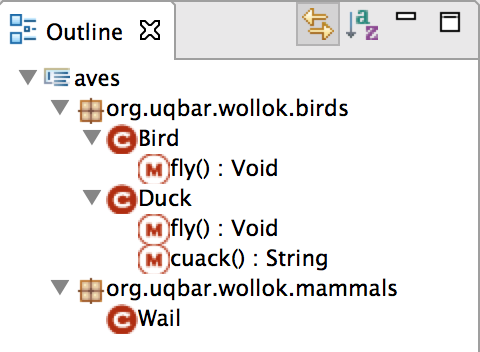
\includegraphics[scale=0.5]{images/wollok-paper-outline.png}
    \caption{Outline View: This view shows the structure of the file.}
    \label{fig:outline.png}
\end{figure}

\begin{figure}[ht]
    \centering
	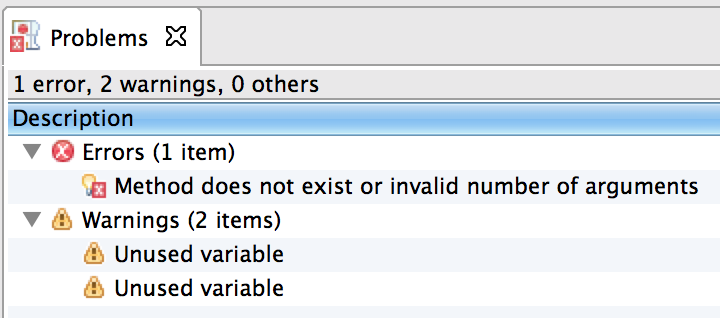
\includegraphics[scale=0.5]{images/wollok-paper-check-problemsview.png}
    \caption{Problems View: shows the different problems detected by the IDE }
    \label{fig:problemsview.png}
\end{figure}

\begin{figure}[ht]
    \centering
	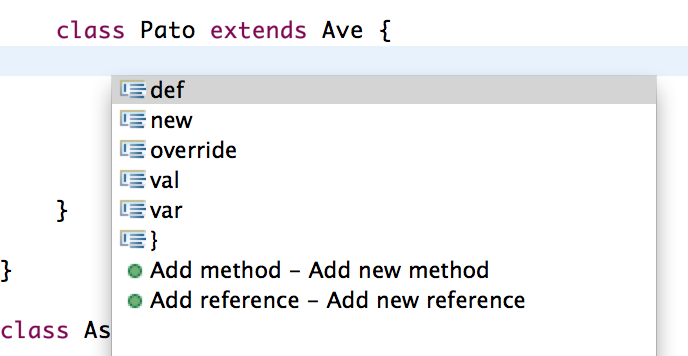
\includegraphics[scale=0.5]{images/wollok-paper-codetemplates.png}
    \caption{Code Assist: code templates for easy edition}
    \label{fig:codetemplates.png}
\end{figure}

\begin{figure}[ht]
    \centering
	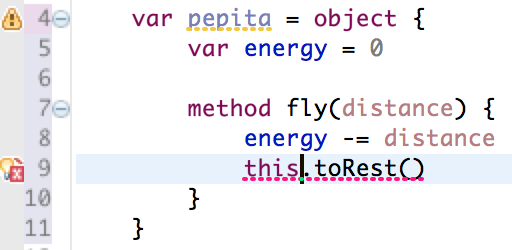
\includegraphics[scale=0.5]{images/wollok-paper-check-noMethodOnThis.png}
    \caption{Detection of an error on sending a message to \emph{this}}
    \label{fig:check-noMethodOnThis.png}
\end{figure}

\begin{figure}[ht]
    \centering
	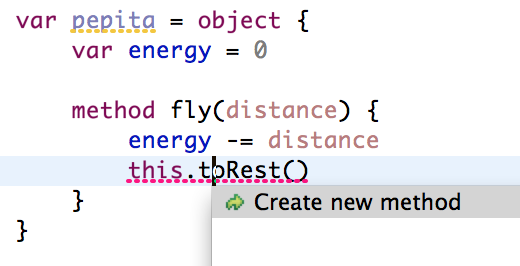
\includegraphics[scale=0.5]{images/wollok-paper-quickfix.png}
    \caption{Quick fix tool for common errors and mistakes}
    \label{fig:quickfix.png}
\end{figure}

\begin{figure}[ht]
    \centering
	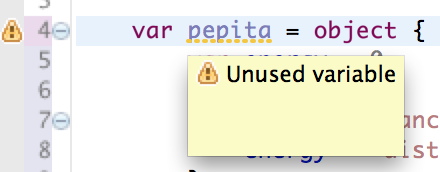
\includegraphics[scale=0.5]{images/wollok-paper-check-unusedVariable.png}
    \caption{Detection of unused variables}
    \label{fig:check-unusedVariable.png}
\end{figure}

\begin{figure}[ht]
    \centering
	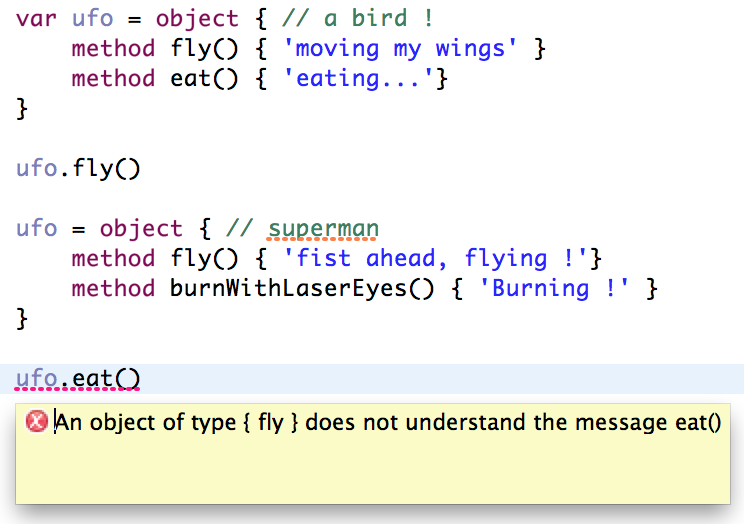
\includegraphics[scale=0.5]{images/wollok-paper-check-messageSending.png}
    \caption{Type system in action, detecting not defined method for the message sent}
    \label{fig:check-messageSending.png}
\end{figure}


\subsection{Software availability}

Wollok is open-sourced and distributed under LGPLv3 License\footnote{http://www.gnu.org/copyleft/lgpl.html}.
Source code and documentation can be found in Bitbucket (\url{https://bitbucket.org/uqbar-project/wollok}) 
And mirrored at Github (\url{https://github.com/uqbar-project/wollok})

\section{Examples of Checks and validations}
\seclabel{ChecksAndValidations}

All the results of the checking and the validation of the program is shown in one integrated view, it is called \emph{Problems}. The figure \figref{problemsview.png} shows a view of this feature. 
There are different types of problems, because these checks and validations are not only used to show type errors or syntax errors, but also to encourage some properties of the program we consider as main topics in the learning process of an OO language.

Here there is a list of all the validations and checking the tool is performing, and a brief reason why they are useful in the teaching of an object oriented language.

\begin{itemize}
  \item \textbf{Syntax Errors}: in this category arises all the errors detected by the parser and the lexical analyser of the language.
  \item \textbf{Style Errors}: this category is useful to teach good practices and to start to talk about code quality, reuse and code sharing.
	\begin{itemize}
		\item \textit{Case in Name}: respecting the difference case conventions for names (\eg using camel case starting with lower case for variables, using camel case starting with upper case for classes).
		\item \textit{Order and grouping}: inside the definition of an object or class the internal references are declared first, then the constructors and finally the methods.
		\item \textit{Modularization}: the classes can only be defined in a library and not in the main program.		
		\item \textit{Duplicated references}: it is impossible to declare a reference using a name already used, this encourage the idea of not having shadowing and improves the readability of the program.
	\end{itemize}
  \item \textbf{References resolution problems}: this errors are useful to detect and avoid references to undeclared variables and also errors in the sending of messages.
  
	\begin{itemize}
	  \item \textit{Undeclared references}: from local variables, parameters or internal fields of objects and classes.
	  \item \textit{Undefined constructors}: checking for the number and type of the parameters.
	  \item \textit{Messages to this}: sending messages to this is a special case, here we can check the existence of the correct method by the number and type of the arguments, even without using type inference.
	\end{itemize}
	
  \item \textbf{Reference usage}: these errors are useful for the detection of erroneous or old code (\eg unused variables or references, sending messages to never assigned variables, using variables instead of values, existence of the overridden method.

  \item \textbf{Type Errors}: the errors are useful for the validation of the compatibility between the references, its possible types, and the messages sent to them, this is performed by the type system and its inferer (\eg message sending, assignation of variables).
\end{itemize}




\end{document}
